\subsubsection{UC15 - Deploy\glo funzione}
\begin{figure}[h]
	\centering
	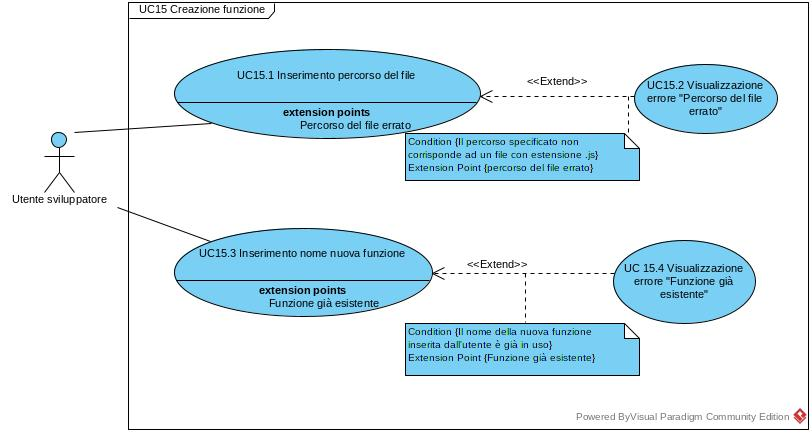
\includegraphics[width=\linewidth]{res/img/UC15.jpg}
	\caption{Diagramma UC15 - Deploy funzione}
\end{figure}
\begin{itemize}
	\item \textbf{Attori primari:} Utente sviluppatore;
	\item \textbf{Descrizione:} l'utente potrà eseguire il \textit{deploy\glo} di una propria funzione JavaScript su \textit{Etherless-server} rendendola disponibile a tutti gli utenti del servizio; 
	\item \textbf{Pre-condizioni:} l'utente possiede una funzione JavaScript sul proprio dispositivo;
	\item \textbf{Post-condizioni:} il sistema si occuperà di creare una nuova istanza su AWS Lambda con il nome specificato e rendere disponibile la sua esecuzione a tutti gli utenti di \textit{Etherless}. L'utente visualizzerà a schermo l'esito del comando;
	\item \textbf{Scenario principale:} 
	\begin{enumerate}
		\item L'utente tramite il comando \textit{"deploy\glos"} crea una nuova istanza della funzione su AWS Lambda;
		\item Il sistema visualizzerà su schermo l'esito dell'operazione.
	\end{enumerate}
\end{itemize}